% Atwood Machines in TikZ (Half Atwood Machine)
% Latexdraw.com
% 26/04/2020, 07:28


\documentclass{standalone}
\usepackage{tikz}
\usetikzlibrary{patterns}

\begin{document}

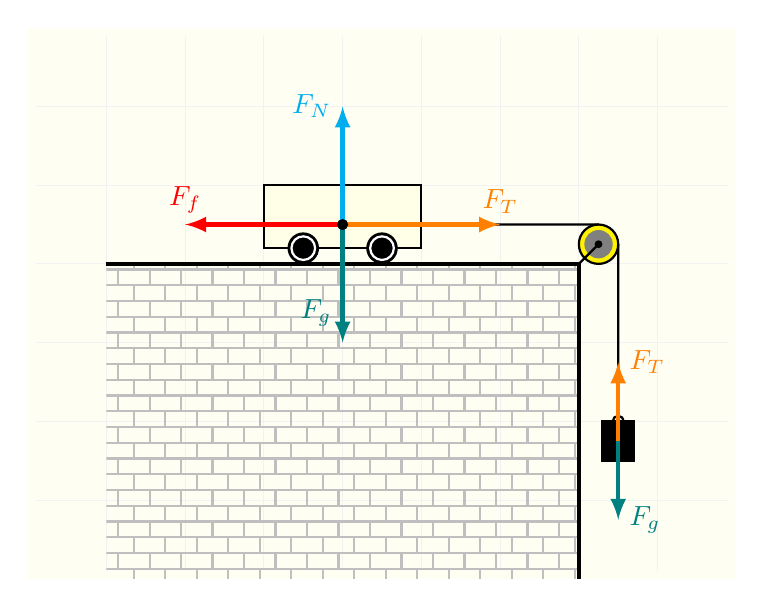
\begin{tikzpicture}[thick] 

% Background
\fill [yellow!5](-3,0) rectangle (6,7);
\draw [gray!10,thin](-2.9,0.1) grid (5.9,6.9);

% Ground
\fill[pattern=bricks,pattern color=lightgray] (-2,4) rectangle (4,0);
\draw[very thick](-2,4) -- ++(6,0) -- ++(0,-4);


% Pulley
\draw[fill=yellow] (4.25,4.25) circle(0.25);
\fill[gray] (4.25,4.25) circle(0.18);
\fill (4.25,4.25) circle(0.05);
\draw (4,4) -- (4.25,4.25);

\draw (2,4.5) -- (4.25,4.5)(4.5,4.25) -- (4.5,2)circle(2pt);

% Cart
\draw[black,fill=yellow!10] (0,4.2) rectangle (2,5);
\fill[black] (0.5,4.2) circle(0.2);
\fill[black] (1.5,4.2) circle(0.2);
\draw[white] (0.5,4.2) circle(0.15);
\draw[white] (1.5,4.2) circle(0.15);

% Mass
\draw[fill=black](4.3,2) rectangle (4.7,1.5);

% Free Body Diagram
\draw[-latex,red,ultra thick] (1,4.5) --(-1,4.5) node[above]{$F_f$};
\draw[-latex,orange,ultra thick] (1,4.5) --(3,4.5) node[above]{$F_T$};
\draw[-latex,teal,ultra thick] (1,4.5) --(1,3) node[near end,left]{$F_g$};
\draw[-latex,cyan,ultra thick] (1,4.5) --(1,6) node[left]{$F_N$};
\fill[black] (1,4.5) circle(2pt);

\draw[-latex,teal,ultra thick] (4.5,1.75) --(4.5,0.75) node[right]{$F_g$};
\draw[-latex,orange,ultra thick] (4.5,1.75) --(4.5,2.75) node[right]{$F_T$};

\end{tikzpicture}


\end{document}
